\documentclass{standalone}
\usepackage{tikz}
\usepackage{xcolor}
\usetikzlibrary{patterns, positioning}
\usetikzlibrary{shapes.misc}
\usepackage[outline]{contour}
\contourlength{1.5pt} 


\begin{document}
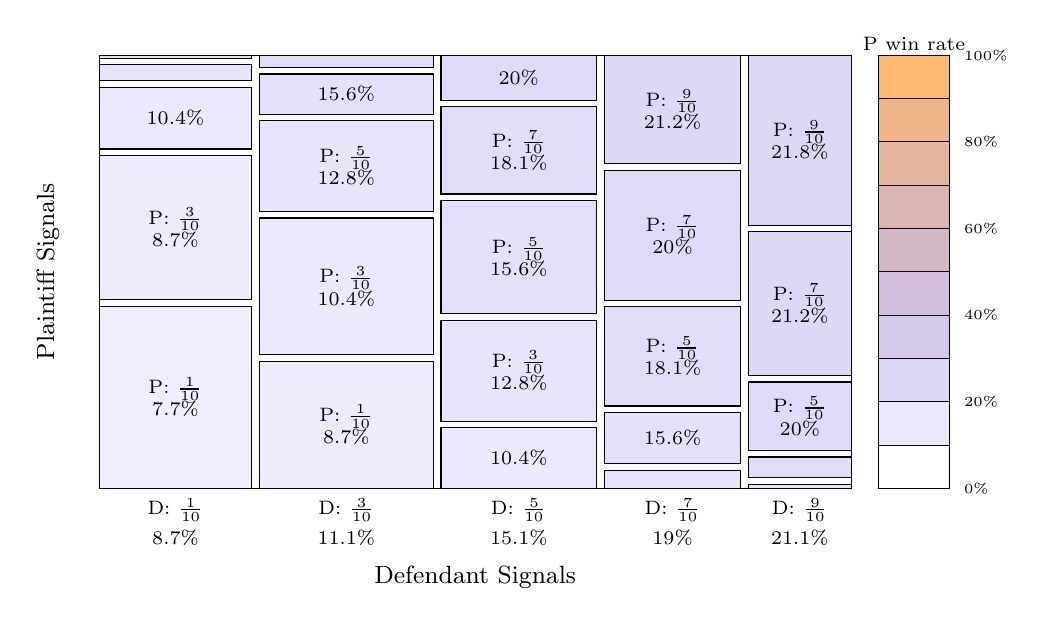
\begin{tikzpicture}
\newcommand{\DFractionOffset}{0.4}
\newcommand{\AxisLabelYAdjust}{-0.235}
\draw[draw=black] (0.6,2) rectangle (10.15,7.5);
\draw[fill=blue!92!orange!8!white!85!white, draw=black] (0.6,2) rectangle (2.5387,4.3147);
\draw (1.5693639169900284, 3.1573581866305807) node[font=\scriptsize, text=black, align=center] {P: $\frac{1}{10}$\\ 7.7\%};
\draw[fill=blue!91!orange!9!white!85!white, draw=black] (0.6,4.3947) rectangle (2.5387,6.2309);
\draw (1.5693639169900284, 5.31281783888332) node[font=\scriptsize, text=black, align=center] {P: $\frac{3}{10}$\\ 8.7\%};
\draw[fill=blue!90!orange!10!white!85!white, draw=black] (0.6,6.3109) rectangle (2.5387,7.0964);
\draw (1.5693639169900284, 6.703654506609724) node[font=\scriptsize, text=black, align=center] {10.4\%};
\draw[fill=blue!87!orange!13!white!84!white, draw=black] (0.6,7.1764) rectangle (2.5387,7.3835);
\draw[fill=blue!84!orange!16!white!83!white, draw=black] (0.6,7.4635) rectangle (2.5387,7.5);
\draw (1.5693639169900284, 1.6) node[anchor=north, font=\scriptsize, text=black] {8.7\%};
\draw (1.5693639169900284, {1.6 + \DFractionOffset}) node[anchor=north, font=\scriptsize, text=black] {D: $\frac{1}{10}$};
\draw[fill=blue!91!orange!9!white!85!white, draw=black] (2.6387,2) rectangle (4.8414,3.6162);
\draw (3.7400723970367635, 2.8080799259041314) node[font=\scriptsize, text=black, align=center] {P: $\frac{1}{10}$\\ 8.7\%};
\draw[fill=blue!90!orange!10!white!85!white, draw=black] (2.6387,3.6962) rectangle (4.8414,5.4344);
\draw (3.7400723970367635, 4.565289769424391) node[font=\scriptsize, text=black, align=center] {P: $\frac{3}{10}$\\ 10.4\%};
\draw[fill=blue!87!orange!13!white!84!white, draw=black] (2.6387,5.5144) rectangle (4.8414,6.6692);
\draw (3.7400723970367635, 6.091825926518461) node[font=\scriptsize, text=black, align=center] {P: $\frac{5}{10}$\\ 12.8\%};
\draw[fill=blue!84!orange!16!white!83!white, draw=black] (2.6387,6.7492) rectangle (4.8414,7.2634);
\draw (3.7400723970367635, 7.00633695761053) node[font=\scriptsize, text=black, align=center] {15.6\%};
\draw[fill=blue!82!orange!18!white!82!white, draw=black] (2.6387,7.3434) rectangle (4.8414,7.5);
\draw (3.7400723970367635, 1.6) node[anchor=north, font=\scriptsize, text=black] {11.1\%};
\draw (3.7400723970367635, {1.6 + \DFractionOffset}) node[anchor=north, font=\scriptsize, text=black] {D: $\frac{3}{10}$};
\draw[fill=blue!90!orange!10!white!85!white, draw=black] (4.9414,2) rectangle (6.9175,2.7706);
\draw (5.929453597504486, 2.385312972653737) node[font=\scriptsize, text=black, align=center] {10.4\%};
\draw[fill=blue!87!orange!13!white!84!white, draw=black] (4.9414,2.8506) rectangle (6.9175,4.1379);
\draw (5.929453597504486, 3.494249064578009) node[font=\scriptsize, text=black, align=center] {P: $\frac{3}{10}$\\ 12.8\%};
\draw[fill=blue!84!orange!16!white!83!white, draw=black] (4.9414,4.2179) rectangle (6.9175,5.6594);
\draw (5.929453597504486, 4.938623371920556) node[font=\scriptsize, text=black, align=center] {P: $\frac{5}{10}$\\ 15.6\%};
\draw[fill=blue!82!orange!18!white!82!white, draw=black] (4.9414,5.7394) rectangle (6.9175,6.8448);
\draw (5.929453597504486, 6.2920891439701645) node[font=\scriptsize, text=black, align=center] {P: $\frac{7}{10}$\\ 18.1\%};
\draw[fill=blue!80!orange!20!white!81!white, draw=black] (4.9414,6.9248) rectangle (6.9175,7.5);
\draw (5.929453597504486, 7.21240186397388) node[font=\scriptsize, text=black, align=center] {20\%};
\draw (5.929453597504486, 1.6) node[anchor=north, font=\scriptsize, text=black] {15.1\%};
\draw (5.929453597504486, {1.6 + \DFractionOffset}) node[anchor=north, font=\scriptsize, text=black] {D: $\frac{5}{10}$};
\draw[fill=blue!87!orange!13!white!84!white, draw=black] (7.0175,2) rectangle (8.7476,2.2321);
\draw[fill=blue!84!orange!16!white!83!white, draw=black] (7.0175,2.3121) rectangle (8.7476,2.9668);
\draw (7.882523211416605, 2.639428032210156) node[font=\scriptsize, text=black, align=center] {15.6\%};
\draw[fill=blue!82!orange!18!white!82!white, draw=black] (7.0175,3.0468) rectangle (8.7476,4.3094);
\draw (7.882523211416605, 3.678077292884027) node[font=\scriptsize, text=black, align=center] {P: $\frac{5}{10}$\\ 18.1\%};
\draw[fill=blue!80!orange!20!white!81!white, draw=black] (7.0175,4.3894) rectangle (8.7476,6.0413);
\draw (7.882523211416605, 5.21532345365786) node[font=\scriptsize, text=black, align=center] {P: $\frac{7}{10}$\\ 20\%};
\draw[fill=blue!79!orange!21!white!81!white, draw=black] (7.0175,6.1213) rectangle (8.7476,7.5);
\draw (7.882523211416605, 6.810630795266999) node[font=\scriptsize, text=black, align=center] {P: $\frac{9}{10}$\\ 21.2\%};
\draw (7.882523211416605, 1.6) node[anchor=north, font=\scriptsize, text=black] {19\%};
\draw (7.882523211416605, {1.6 + \DFractionOffset}) node[anchor=north, font=\scriptsize, text=black] {D: $\frac{7}{10}$};
\draw[fill=blue!84!orange!16!white!83!white, draw=black] (8.8476,2) rectangle (10.15,2.0543);
\draw[fill=blue!82!orange!18!white!82!white, draw=black] (8.8476,2.1343) rectangle (10.15,2.3991);
\draw[fill=blue!80!orange!20!white!81!white, draw=black] (8.8476,2.4791) rectangle (10.15,3.3518);
\draw (9.498778093958855, 2.915451196732595) node[font=\scriptsize, text=black, align=center] {P: $\frac{5}{10}$\\ 20\%};
\draw[fill=blue!79!orange!21!white!81!white, draw=black] (8.8476,3.4318) rectangle (10.15,5.2632);
\draw (9.498778093958855, 4.347501215559324) node[font=\scriptsize, text=black, align=center] {P: $\frac{7}{10}$\\ 21.2\%};
\draw[fill=blue!78!orange!22!white!81!white, draw=black] (8.8476,5.3432) rectangle (10.15,7.5);
\draw (9.498778093958855, 6.421603061410659) node[font=\scriptsize, text=black, align=center] {P: $\frac{9}{10}$\\ 21.8\%};
\draw (9.498778093958855, 1.6) node[anchor=north, font=\scriptsize, text=black] {21.1\%};
\draw (9.498778093958855, {1.6 + \DFractionOffset}) node[anchor=north, font=\scriptsize, text=black] {D: $\frac{9}{10}$};
\node[font=\small, text=black] at (5.375, {1.1 + \AxisLabelYAdjust}) {Defendant Signals};
\node[font=\small, text=black, rotate=90] at (-0.050000000000000044, 4.75) {Plaintiff Signals};
\draw[draw=black] (10.5,2) rectangle (11.4,7.5);
\draw (10.95, 7.65) node[font=\scriptsize, text=black] {P win rate};
\draw[fill=blue!100!orange!0!white!88!white, draw=black] (10.5,2) rectangle (11.4,2.55);
\draw[fill=blue!89!orange!11!white!84!white, draw=black] (10.5,2.55) rectangle (11.4,3.1);
\draw[fill=blue!78!orange!22!white!81!white, draw=black] (10.5,3.1) rectangle (11.4,3.65);
\draw[fill=blue!67!orange!33!white!77!white, draw=black] (10.5,3.65) rectangle (11.4,4.2);
\draw[fill=blue!56!orange!44!white!73!white, draw=black] (10.5,4.2) rectangle (11.4,4.75);
\draw[fill=blue!44!orange!56!white!70!white, draw=black] (10.5,4.75) rectangle (11.4,5.3);
\draw[fill=blue!33!orange!67!white!66!white, draw=black] (10.5,5.3) rectangle (11.4,5.85);
\draw[fill=blue!22!orange!78!white!62!white, draw=black] (10.5,5.85) rectangle (11.4,6.4);
\draw[fill=blue!11!orange!89!white!59!white, draw=black] (10.5,6.4) rectangle (11.4,6.95);
\draw[fill=blue!0!orange!100!white!55!white, draw=black] (10.5,6.95) rectangle (11.4,7.5);
\draw (11.46, 2) node[anchor=west, font=\tiny, text=black] {0\%};
\draw (11.46, 3.1) node[anchor=west, font=\tiny, text=black] {20\%};
\draw (11.46, 4.2) node[anchor=west, font=\tiny, text=black] {40\%};
\draw (11.46, 5.3) node[anchor=west, font=\tiny, text=black] {60\%};
\draw (11.46, 6.4) node[anchor=west, font=\tiny, text=black] {80\%};
\draw (11.46, 7.5) node[anchor=west, font=\tiny, text=black] {100\%};


\end{tikzpicture}
\end{document}